% Options for packages loaded elsewhere
\PassOptionsToPackage{unicode}{hyperref}
\PassOptionsToPackage{hyphens}{url}
%
\documentclass[
  9pt,
  ignorenonframetext,
]{beamer}
\usepackage{pgfpages}
\setbeamertemplate{caption}[numbered]
\setbeamertemplate{caption label separator}{: }
\setbeamercolor{caption name}{fg=normal text.fg}
\beamertemplatenavigationsymbolshorizontal
% Prevent slide breaks in the middle of a paragraph
\widowpenalties 1 10000
\raggedbottom
\setbeamertemplate{part page}{
  \centering
  \begin{beamercolorbox}[sep=16pt,center]{part title}
    \usebeamerfont{part title}\insertpart\par
  \end{beamercolorbox}
}
\setbeamertemplate{section page}{
  \centering
  \begin{beamercolorbox}[sep=12pt,center]{part title}
    \usebeamerfont{section title}\insertsection\par
  \end{beamercolorbox}
}
\setbeamertemplate{subsection page}{
  \centering
  \begin{beamercolorbox}[sep=8pt,center]{part title}
    \usebeamerfont{subsection title}\insertsubsection\par
  \end{beamercolorbox}
}
\AtBeginPart{
  \frame{\partpage}
}
\AtBeginSection{
  \ifbibliography
  \else
    \frame{\sectionpage}
  \fi
}
\AtBeginSubsection{
  \frame{\subsectionpage}
}

\usepackage{amsmath,amssymb}
\usepackage{iftex}
\ifPDFTeX
  \usepackage[T1]{fontenc}
  \usepackage[utf8]{inputenc}
  \usepackage{textcomp} % provide euro and other symbols
\else % if luatex or xetex
  \usepackage{unicode-math}
  \defaultfontfeatures{Scale=MatchLowercase}
  \defaultfontfeatures[\rmfamily]{Ligatures=TeX,Scale=1}
\fi
\usepackage{lmodern}
\ifPDFTeX\else  
    % xetex/luatex font selection
\fi
% Use upquote if available, for straight quotes in verbatim environments
\IfFileExists{upquote.sty}{\usepackage{upquote}}{}
\IfFileExists{microtype.sty}{% use microtype if available
  \usepackage[]{microtype}
  \UseMicrotypeSet[protrusion]{basicmath} % disable protrusion for tt fonts
}{}
\makeatletter
\@ifundefined{KOMAClassName}{% if non-KOMA class
  \IfFileExists{parskip.sty}{%
    \usepackage{parskip}
  }{% else
    \setlength{\parindent}{0pt}
    \setlength{\parskip}{6pt plus 2pt minus 1pt}}
}{% if KOMA class
  \KOMAoptions{parskip=half}}
\makeatother
\usepackage{xcolor}
\newif\ifbibliography
\setlength{\emergencystretch}{3em} % prevent overfull lines
\setcounter{secnumdepth}{-\maxdimen} % remove section numbering


\providecommand{\tightlist}{%
  \setlength{\itemsep}{0pt}\setlength{\parskip}{0pt}}\usepackage{longtable,booktabs,array}
\usepackage{calc} % for calculating minipage widths
\usepackage{caption}
% Make caption package work with longtable
\makeatletter
\def\fnum@table{\tablename~\thetable}
\makeatother
\usepackage{graphicx}
\makeatletter
\def\maxwidth{\ifdim\Gin@nat@width>\linewidth\linewidth\else\Gin@nat@width\fi}
\def\maxheight{\ifdim\Gin@nat@height>\textheight\textheight\else\Gin@nat@height\fi}
\makeatother
% Scale images if necessary, so that they will not overflow the page
% margins by default, and it is still possible to overwrite the defaults
% using explicit options in \includegraphics[width, height, ...]{}
\setkeys{Gin}{width=\maxwidth,height=\maxheight,keepaspectratio}
% Set default figure placement to htbp
\makeatletter
\def\fps@figure{htbp}
\makeatother

\titlegraphic{
\begin{minipage}{0.4\linewidth}
    \includegraphics[width=\linewidth]{reichlab.png}
\end{minipage}%
\hspace{0.06\linewidth}
\begin{minipage}{0.4\linewidth}
    \includegraphics[width=\linewidth]{C19FH.png}
\end{minipage}%
}
\makeatletter
\makeatother
\makeatletter
\makeatother
\makeatletter
\@ifpackageloaded{caption}{}{\usepackage{caption}}
\AtBeginDocument{%
\ifdefined\contentsname
  \renewcommand*\contentsname{Table of contents}
\else
  \newcommand\contentsname{Table of contents}
\fi
\ifdefined\listfigurename
  \renewcommand*\listfigurename{List of Figures}
\else
  \newcommand\listfigurename{List of Figures}
\fi
\ifdefined\listtablename
  \renewcommand*\listtablename{List of Tables}
\else
  \newcommand\listtablename{List of Tables}
\fi
\ifdefined\figurename
  \renewcommand*\figurename{Figure}
\else
  \newcommand\figurename{Figure}
\fi
\ifdefined\tablename
  \renewcommand*\tablename{Table}
\else
  \newcommand\tablename{Table}
\fi
}
\@ifpackageloaded{float}{}{\usepackage{float}}
\floatstyle{ruled}
\@ifundefined{c@chapter}{\newfloat{codelisting}{h}{lop}}{\newfloat{codelisting}{h}{lop}[chapter]}
\floatname{codelisting}{Listing}
\newcommand*\listoflistings{\listof{codelisting}{List of Listings}}
\makeatother
\makeatletter
\@ifpackageloaded{caption}{}{\usepackage{caption}}
\@ifpackageloaded{subcaption}{}{\usepackage{subcaption}}
\makeatother
\makeatletter
\@ifpackageloaded{tcolorbox}{}{\usepackage[skins,breakable]{tcolorbox}}
\makeatother
\makeatletter
\@ifundefined{shadecolor}{\definecolor{shadecolor}{rgb}{.97, .97, .97}}
\makeatother
\makeatletter
\makeatother
\makeatletter
\makeatother
\ifLuaTeX
  \usepackage{selnolig}  % disable illegal ligatures
\fi
\IfFileExists{bookmark.sty}{\usepackage{bookmark}}{\usepackage{hyperref}}
\IfFileExists{xurl.sty}{\usepackage{xurl}}{} % add URL line breaks if available
\urlstyle{same} % disable monospaced font for URLs
\hypersetup{
  pdfauthor={Aaron Gerding, Nick Reich, Ben Rogers, Evan Ray},
  hidelinks,
  pdfcreator={LaTeX via pandoc}}

\title{Infectious Disease Forecast Evaluation Via Social Utility:
Allocation Scores}
\subtitle{MIDAS 2023}
\author{Aaron Gerding, Nick Reich, Ben Rogers, Evan Ray}
\date{}
\institute{School of Public Health and Health Sciences, UMass, Amherst\\
Department of Biostatistics and Epidemiology}

\begin{document}
\frame{\titlepage}
\ifdefined\Shaded\renewenvironment{Shaded}{\begin{tcolorbox}[boxrule=0pt, breakable, interior hidden, sharp corners, frame hidden, borderline west={3pt}{0pt}{shadecolor}, enhanced]}{\end{tcolorbox}}\fi

\begin{frame}{Outbreak Forecast Hubs and \textbf{Informed} Resource
Allocation}
\protect\hypertarget{outbreak-forecast-hubs-and-informed-resource-allocation}{}
Hubs developed to \textbf{``inform public health responses''}

\begin{itemize}
\item
  such as how resources are \textbf{allocated} among locations
\item
  e.g., medical supplies, facility capacity, personnel
\end{itemize}

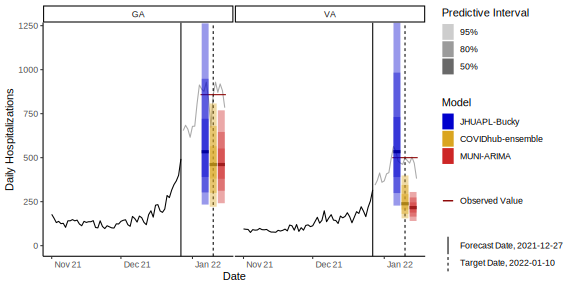
\includegraphics{../plots/output/p_VA_JHU_MUNI.jpeg}

\note{quantiles flexible interpretable - closer to describing full
distribution which DM probably always wants

multicenter effort to collect forecasts via hubs for ID outbreaks
(epi/pan/endemic)

With uncertainty quantification being well-established as needed DM
input,

Allocations can be wrt space, time, demographic

Next: formalize this.}
\end{frame}

\begin{frame}{Scoring rules and social welfare}
\protect\hypertarget{scoring-rules-and-social-welfare}{}
Hubs strive to rank and combine forecasts so as to optimize social
welfare via the public health decisions that forecasts inform

\begin{itemize}
\item
  uncertainty quantification, and therefore, probabilistic forecasting
  essential
\item
  basic strategy: use a \textbf{scoring rule} \(S\) which assigns a loss
  \(S(F,y)\) when a probabilistic forecast \(F\) of \(Y\) is chosen and
  \(Y=y\) is observed.
\item
  optimizing welfare requires that forecasters say what they believe; so
  \(S\) should be \textbf{proper} meaning
  \(\displaystyle{E_{F}[S(F,Y)] \leq E_{F}S(G,Y)]}\) for all \(F, G\)
\end{itemize}

Current standard is the \textbf{Weighted Interval Score} (discrete CRPS)

\begin{itemize}
\tightlist
\item
  adopted largely for convenient scoring of quantile forecasts.
\end{itemize}
\end{frame}

\begin{frame}{Tools from decision theory}
\protect\hypertarget{tools-from-decision-theory}{}
\begin{block}{A central goal in design of scoring rules}
\protect\hypertarget{a-central-goal-in-design-of-scoring-rules}{}
Tie forecast scores directly to the benefits to society of the decisions
they inform

Key tools from decision theory for linking success/failure of
forecast-informed policy actions to scoring rules:

\begin{itemize}
\item
  Let \(l(x,y)\) be the \textbf{loss} of experiencing \(y\) after taking
  policy action \(x\)
\item
  The \textbf{Bayes risk} of a forecast \(Y \sim F\) is
  \(\min_x E_F[l(x,Y)]\)
\item
  A \textbf{Bayes act} for \(F\) is an action \(x^F\) that attains this
  minimum
\item
  Losses from Bayes acts define an \emph{automatically proper} scoring
  rule
\end{itemize}

\[
S(F,y) := l(x^F, y)
\]

\textbf{Note:} Scoring rules are really only a means to an end. It is
the expected score, in this case the Bayes risk, which characterize the
value a forecast adds for a decision maker. Scoring rule sample averages
estimate the expected score.
\end{block}
\end{frame}

\begin{frame}{A new scoring rule via a new loss function for constrained
actions}
\protect\hypertarget{a-new-scoring-rule-via-a-new-loss-function-for-constrained-actions}{}
\begin{block}{Our basic example:}
\protect\hypertarget{our-basic-example}{}
\begin{itemize}
\item
  \(x\) and \(y\) are vectors in \(\mathbb{N}_0^{52}\)
\item
  \(y =\) number of severe cases in US states and territories
\item
  \(l(x,y) =\) unmet need when \(x\) beds allocated and \(y\) severe
  cases occur
\end{itemize}

\begin{align*}
l(x,y) &= \sum_{i=1}^{52} \max(y_i - x_i, 0)\\
x^F &= \text{minimizer of } E_{F}[l(x,Y)] \text{ over all feasible } x
\end{align*} 

\textbf{Our new idea:} Define \textbf{feasible} \(x\) as satisfying
\(\displaystyle{\sum x_i \leq K}\)

\note{social/political/economic/psychological/moral utility

this must somehow acknowledge risk attitude heterogeneity among various
DM's that a forecast hub might serve

gpl parameters, weights, multiple constraints}
\end{block}
\end{frame}

\begin{frame}{Computation}
\protect\hypertarget{computation}{}
Obtaining \(x^F\) is a constrained stochastic optimization problem

\begin{itemize}
\item
  known in inventory management as a \textbf{constrained multi-product
  newsvendor} problem
\item
  formally solvable using Lagrange multiplier method to get a quantile
  representation \(x_i^F = F_i^{-1}(\tau(K,F)), i = 1,\ldots,N\)
\item
  in practice, we find \(x_i^F\)'s via an iterative method:
\end{itemize}

\includegraphics{../plots/output/iter_combo.png}
\end{frame}

\begin{frame}{Application}
\protect\hypertarget{application}{}
December 2021: Omicron wave clearly started US but forecast teams unsure
of severity given uncertainty about \(R_0\), cross-protection by
vaccination, previous infection, etc.

\includegraphics{../plots/output/nat_hosps.png}
\end{frame}

\begin{frame}{Oracle adjusted allocation scores near Omicron peak}
\protect\hypertarget{oracle-adjusted-allocation-scores-near-omicron-peak}{}
\includegraphics{../plots/output/peak_alloscore.png}
\end{frame}

\begin{frame}{Some Observations}
\protect\hypertarget{some-observations}{}
\begin{columns}[T]
\begin{column}{0.4\textwidth}
\begin{itemize}
\item
  related to the Murphy curves of Ehm, Gneiting, Jordan, Krüger, 2016
\item
  extreme shortage or surplus diminishes oracle's advantage
\item
  ranking consistent across large \(K\) region.
\end{itemize}
\end{column}

\begin{column}{0.6\textwidth}
\includegraphics{../plots/output/peak_alloscore_min.png}
\end{column}
\end{columns}
\end{frame}

\begin{frame}{Alloscore and WIS rank models differently}
\protect\hypertarget{alloscore-and-wis-rank-models-differently}{}
\includegraphics{../plots/output/p_wis_v_alloscore.png}
\end{frame}

\begin{frame}{Explanations?}
\protect\hypertarget{explanations}{}
\includegraphics{../plots/output/mvbucky_dist_alloc.png}
\end{frame}

\begin{frame}[fragile]{Limitations}
\protect\hypertarget{limitations}{}
This is \textbf{post-hoc} analysis

Hub forecasters were unaware of

\begin{itemize}
\item
  an allocation score (on joint forecast)
\item
  any allocation based loss
\item
  our quantile interpolation/extrapolation methods (\texttt{distfromq})

  \begin{itemize}
  \tightlist
  \item
    might be especially important for tails
  \end{itemize}
\end{itemize}

We hope/think that allocation scoring is sensitive to implicit
dependence structures in forecasts, but all work so far only refers
directly to marginals - nothing yet with copulas, etc.

\begin{block}{Thank you!}
\protect\hypertarget{thank-you}{}
A very rough R package I wrote to implement scoring procedures:

\url{https://github.com/aaronger/alloscore}

A less rough package Evan wrote to implement cdf reconstruction

\url{https://github.com/reichlab/distfromq}
\end{block}
\end{frame}



\end{document}
